\documentclass[12pt,oneside,a4paper]{book}
\usepackage{mathtools}
\usepackage[top=2.5cm,bottom=2.5cm,right=2cm,left=3.5cm]{geometry}
\usepackage[utf8]{inputenc}
\usepackage{graphicx}
\usepackage{pdfpages}
%\usepackage{lmodern}
\usepackage{txfonts} %Times New Roman
\usepackage[T1]{fontenc}
\usepackage[english,slovak]{babel}
\usepackage{amsmath}
\usepackage{amssymb}
\usepackage{mathrsfs}
\linespread{1.3} %riadkovanie 1.5
\input foja
\DeclareMathOperator{\lcm}{lcm}
\allowbreak
\begin{document}

%informacie o praci, autorovi,...
\def\school{Comenius University, Bratislava}
\def\faculty{Faculty of Mathematics, Physics and Informatics}
\def\title{Complexity of Language Transformations}
\def\thesis{Diploma Thesis}
\def\author{Boris Vida}
\def\year{2014}
\def\placeandyear{Bratislava, \year}
\def\supervisor{Prof. RNDr. Branislav Rovan, PhD.\ }
\def\studyprogramme{Computer Science}
\def\studyfield{2508 Computer Science, Informatics}
\def\department{Department of Computer Science}

\pdfinfo{/Author (\author) /Title (\title)}

\selectlanguage{english}
\frontmatter
%OBAL
\thispagestyle{empty}
\begin{center}
  \textsc{ 
    {\Large \school\\ \faculty}
    \vfill
    {\LARGE \title}\\ \vspace{0.5cm}
    {\large \thesis}
  }
\end{center}
\vfill

\begin{flushleft}
  \year\\
  \hspace{0.5cm} \author
\end{flushleft}


%TITULNY LIST
\thispagestyle{empty}
\begin{center}
  \textsc{ 
    {\Large \school\\ \faculty}
    \vfill
    {\LARGE \title}\\ \vspace{0.5cm}
    {\large \thesis}
  }
\end{center}
\vfill

\begin{flushleft}
  \begin{tabular}{@{}ll}
    Study programme: & \studyprogramme \\
    Study field: & \studyfield \\
	  Department: & \department \\
    Supervisor: & \supervisor
  \end{tabular}
  \vspace{1cm}

  \placeandyear\\
  \hspace{0.5cm} \author
\end{flushleft}



\shorthandoff{-} %docasne deaktivuje znak '-' v balicku babel
%ZADANIE EN
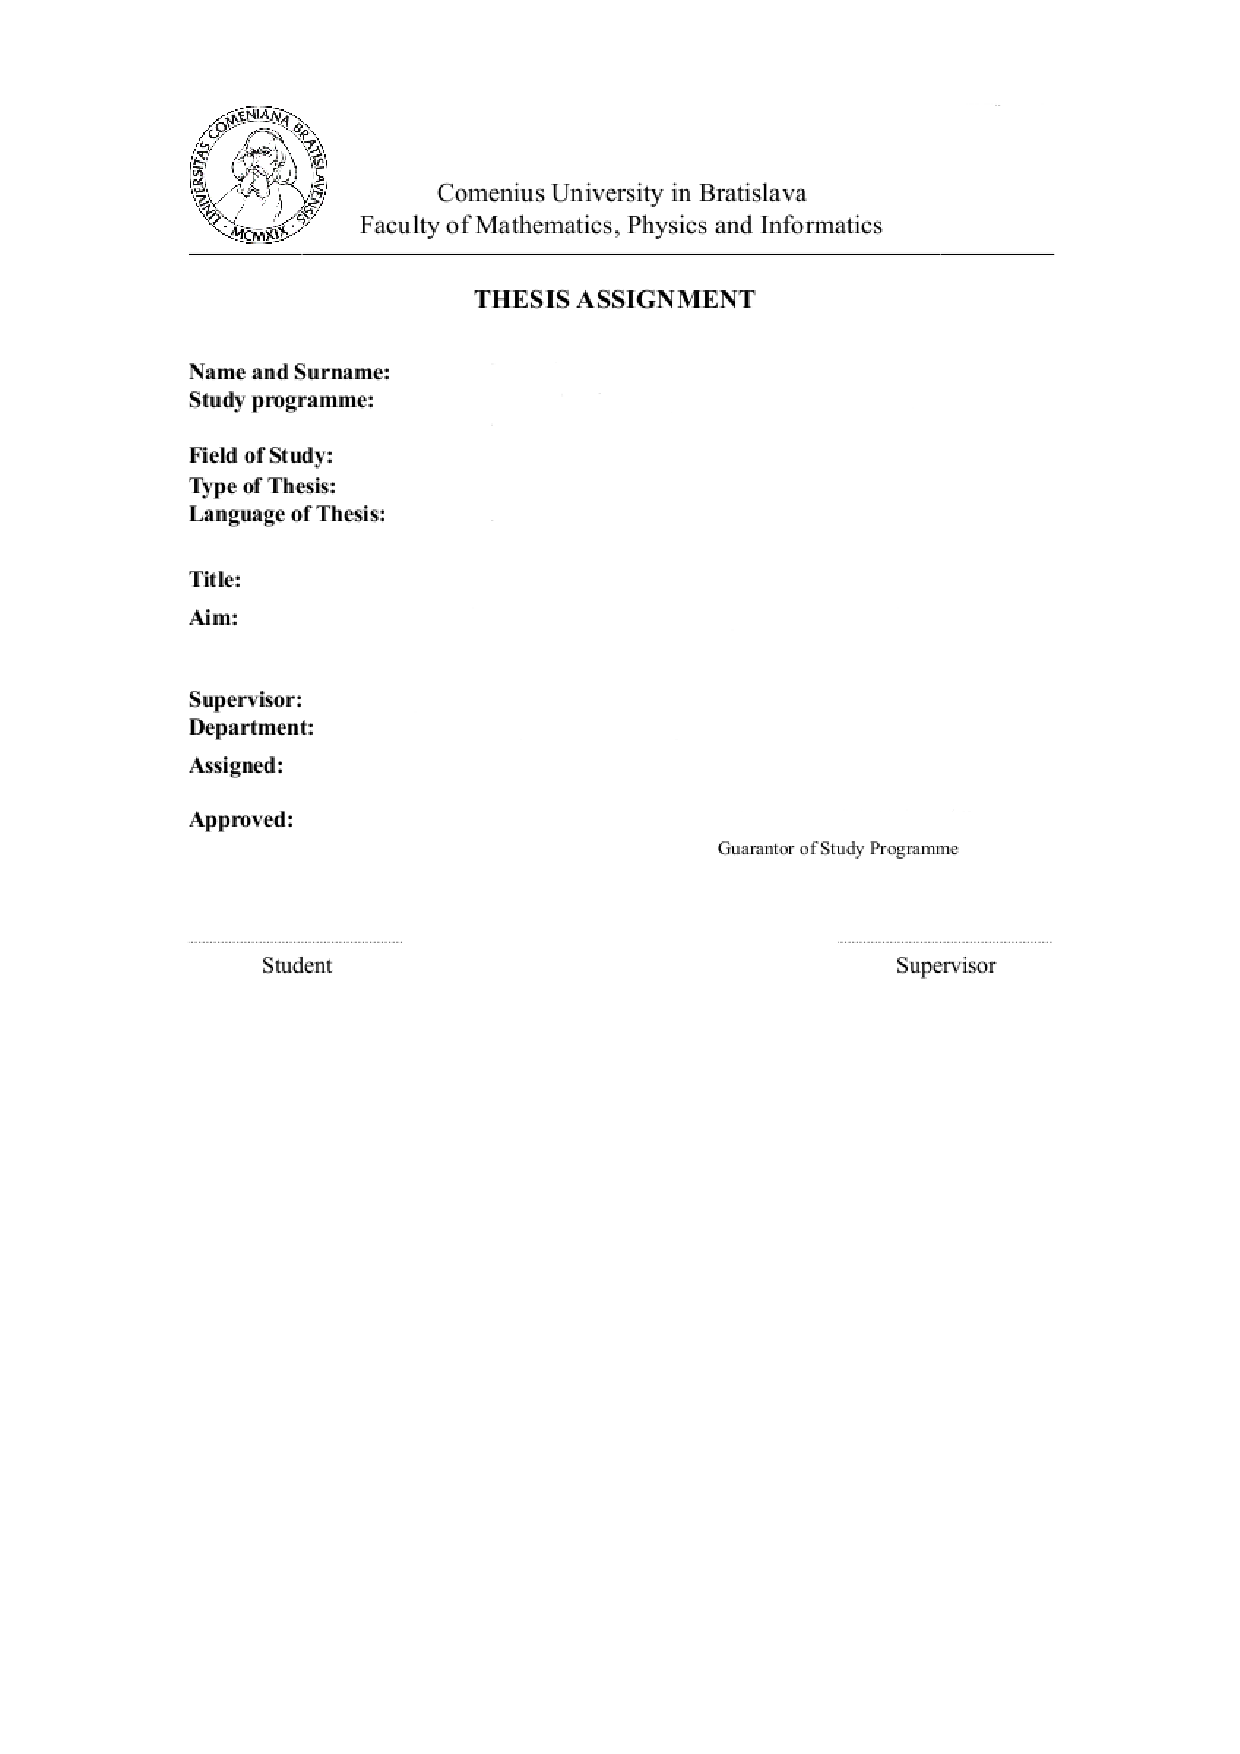
\includepdf[pages=-]{frontmatter/assignment.pdf}
%ZADANIE SK
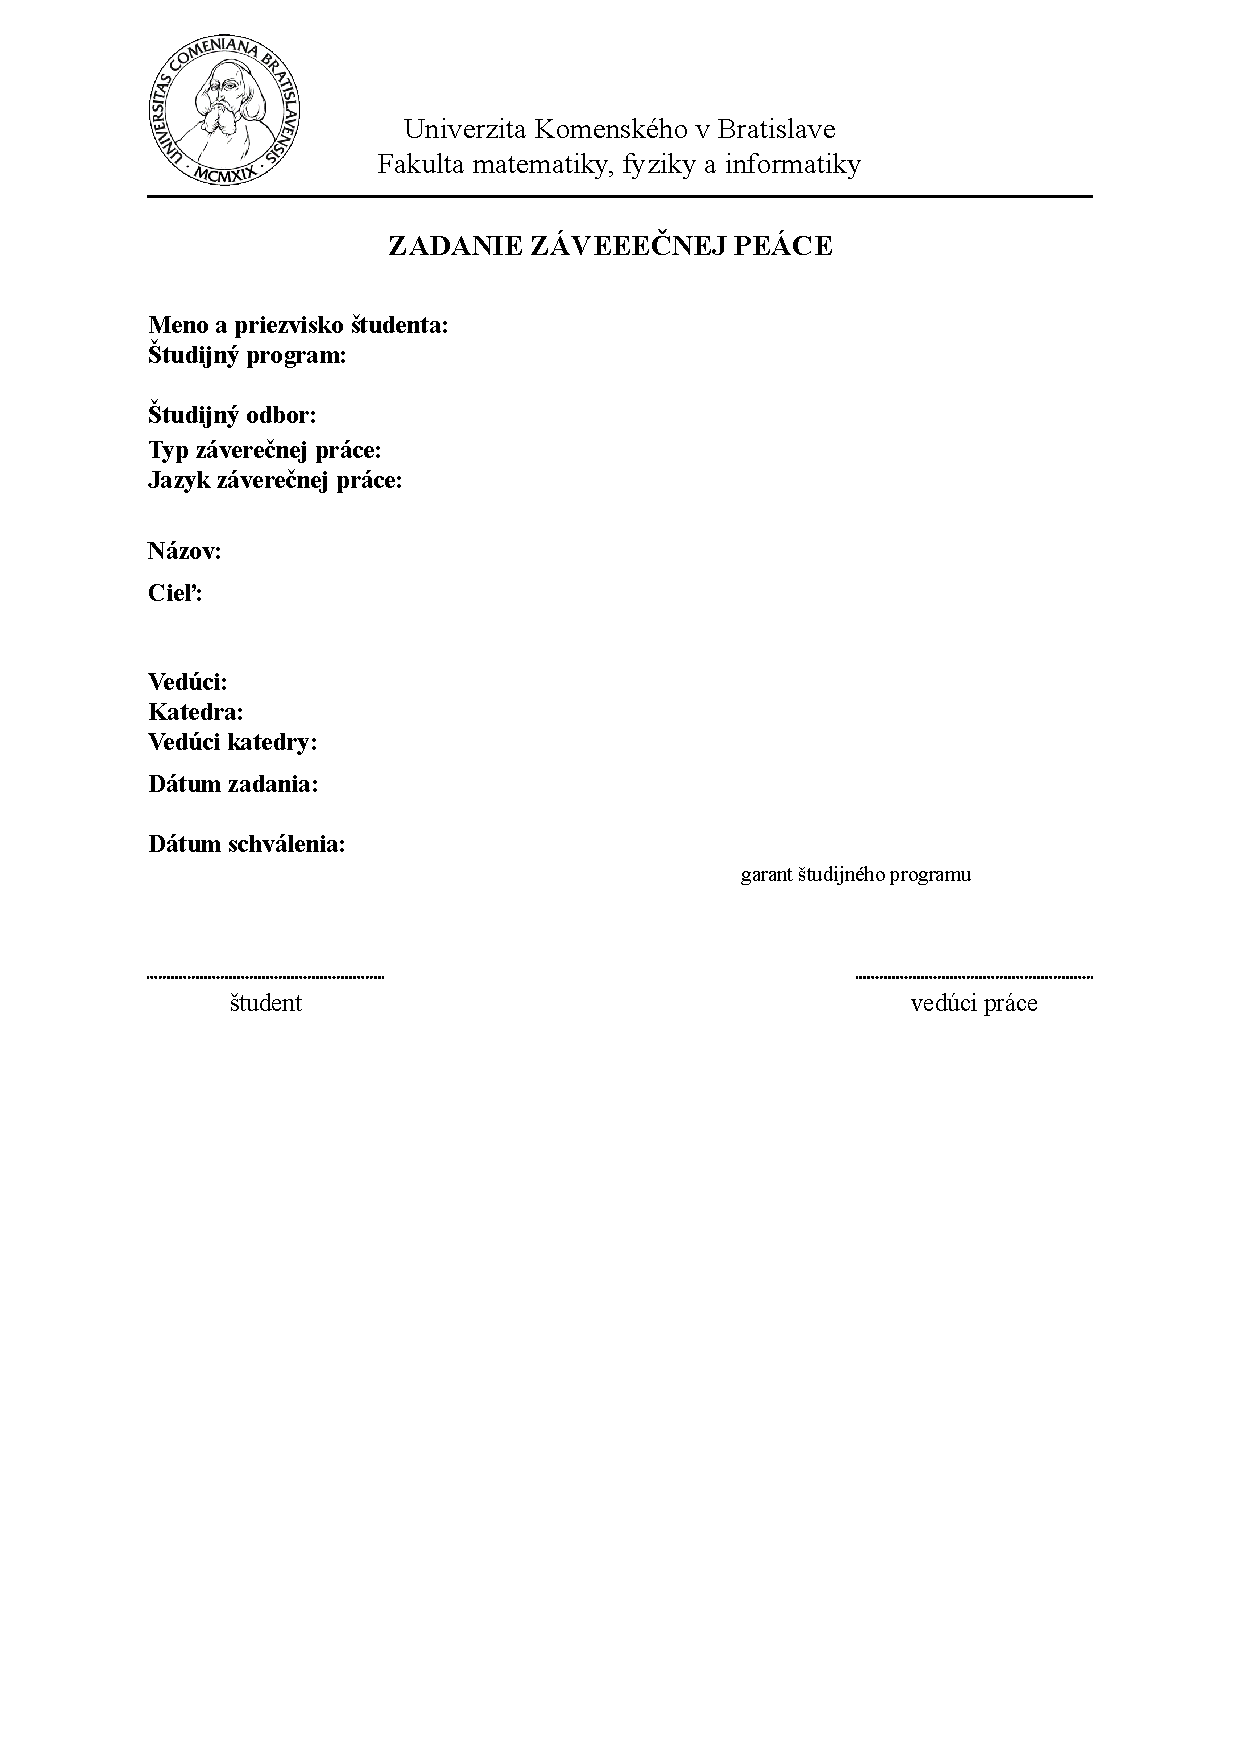
\includepdf[pages=-]{frontmatter/zadanie.pdf}
\shorthandon{-}

%PODAKOVANIE
\chapter*{Acknowledgement}
\vfil
I would like to express gratitude to my supervisor \supervisor for his help and advices by writing of this thesis. I would also like to thank my family and friends for their support during my studies.


%ABSTRAKT SK
\selectlanguage{slovak}
\chapter*{Abstrakt} 
ToDo: Abstrakt
\\
\\
\textbf{\textsc{Keywords:}} transformácie jazykov, popisná zložitosť, a-prekladač


%ABSTRAKT EN
\selectlanguage{english}
\chapter*{Abstract}
ToDo: Abstract
\\
\\
\textbf{\textsc{Keywords:}} language transformations, descriptional complexity, a-transducer


%OBSAH
\tableofcontents

%ZOZNAM ILUSTRACII
%\listoffigures


\mainmatter
\chapter*{Introduction}
\addcontentsline{toc}{chapter}{Introduction}  
\paragraph{}
A number of models for realization of language transformations were introduced in the past fifty years. Most of them can be described as an extension of a finite automaton, which has been augmented by an output tape. Such models are, e. g., Moore and Mealy machines, sequential transducers, general sequential machines, a-transducers, etc.

\paragraph{}
In our thesis, we would like to investigate some complexity properties of these transformation models, with emphasis on a-transducers. 

\paragraph{}
We assume, that the reader is familiar with the basic concepts of formal languages. If this is not the case, we recommend to obtain this understanding from \cite{hopcroft:fola}.


\chapter{Preliminaries}
\label{chap:Preliminaries}

\paragraph{}
In this section, we would like to clarify some basic notations and terminology used in our thesis.

\section{Basic concepts and notation}

%\paragraph{}
%\definicia An \emph{alphabet} is a finite (if not otherwise stated) set of symbols, usually denoted as $\Sigma $. We usually denote members of $\Sigma $ by smallcase letters %from the beginning of the english alphabet, such as $a, b, a_{1}, a_{2},$ etc.

%\paragraph{}
%\definicia A \emph{word} over alphabet $\Sigma $ is a finite sequence of symbols from $\Sigma $. The words are usually denoted by smallcase letters from the end of the english alphabet, such as $u, w, u_{1},$ etc, where e. g. $w \equiv a_{1}a_{2}...a_{n}$ means, that $w$ is formed by a sequence of symbols $a_{1}, a_{2}$ through $a_{n}$.

%\paragraph{}
%\definicia A \emph{language} is any (finite or infinite) set of words over an alphabet $\Sigma $.

\paragraph{}
\oznacenie We denote 
\begin{itemize}
\item by $\epsilon $ an empty string,
\item by $|w|$ the length of a word $w$ ($|\epsilon |=0$),
\item by $|A|$ the number of elements of a finite set (or a finite language) $A$,
\item by $\# _{a}(w)$ the number of symbols $a$ in a word $w$,
\item if $u \equiv a_{1}a_{2}...a_{m}$, $v \equiv b_{1}b_{2}...b_{n}$, then by $u.v$ or simply $uv$ we denote a word $a_{1}a_{2}...a_{m}b_{1}b_{2}...b_{n}$,
\item by $A^{+}$ we denote a transitive closure of $A$, by $A^{*}$ a reflexive-transitive closure of $A$.
\end{itemize}

\paragraph{}
\definicia A \emph{family of languages} is an ordered pair $(\Sigma ,\mathcal{L} )$, such that
\begin{enumerate}
\item $\Sigma $ is an infinite set of symbols
\item every $L\in \mathcal{L} $ is a language over some finite set $\Sigma ^{*} \subset \Sigma $
\item $L \neq \es $ for some $L \in \mathcal{L} $
\end{enumerate}

\paragraph{}
\definicia A \emph{homomorphism} is a function $h: \Sigma_{1}^{*} \rightarrow \Sigma_{2}^{*}$, such that \\	
\centerline{$h(uv) = h(u)h(v)$}

\paragraph{}
\oznacenie If $\forall w \neq \epsilon : h(w) \neq \epsilon $, we call $h$ an \emph{$\epsilon $-free homomorphism} and denote it by $h_{\epsilon }$.

\paragraph{}
\oznacenie For a set $A$, $2^{A}$ is the set of all subsets of $A$.

\paragraph{}
\definicia An \emph{inverse homomorphism} is a function $h^{-1}: \Sigma_{1}^{*} \rightarrow 2^{\Sigma_{2}^{*}}$, such that $h$ is a homomorphism and \\
\centerline{$h^{-1}(u) = \{ v | h(v) = u \} $}

\paragraph{}
\definicia A family of languages is called a \emph{(full) trio}, if it is closed under $\epsilon $-free (arbitrary) homomorphism, inverse homomorphism and intersection with a regular set.

\paragraph{}
\definicia A (full) trio is called a \emph{(full) semi-AFL}, if it is closed under union.

\paragraph{}
\definicia A (full) semi-AFL is called a \emph{(full) AFL}, if it is closed under concatenation and $+$.

\paragraph{}
We now characterize two common used families of language, included in a Chomsky hierarchy, to make clear the notation in this thesis.

\paragraph{}
\oznacenie The family of \emph{regular languages}, denoted by $\R $, is the family of all languages generated by a type 3 grammar or accepted by a deterministic finite automaton (see e. g. \cite{hopcroft:fola} for full definition).

\paragraph{}
\oznacenie The family of \emph{context free languages}, denoted by $\CF $, is the family of all languages generated by a type 2 grammar or accepted by a pushdown finite automaton (see e. g. \cite{hopcroft:fola} for full definition).

\section{Transformation models}
\paragraph{}
Now we would like to define some of the models mentioned in the introduction. Although the central point of our interest is an a-transducer, we also introduce the definitions of other models, which will be used in the next chapters, because they can give us an insight of language transformations in general and many of the concepts used in results involving them can be put to use by examination of a-transducers.

\paragraph{}
Since a-transducer is the most general type of transducer, we define it first and then we only specify the differences between a-transducers and other models.

\paragraph{}
\definicia An \emph{a-transducer} is a 6-tuple $M=(K, \Sigma_{1}, \Sigma_{2}, H, q_{0}, F)$, where
\begin{itemize}
\item $K$ is a finite set of states,
\item $\Sigma_{1} $ and $\Sigma_{2} $ are the input and output alphabet, respectively,
\item $H \subseteq K \times \Sigma_{1}^{*} \times \Sigma_{2}^{*} \times K$ is the transition function, where $H$ is finite,
\item $q_{0} \in K$ is the initial state,
\item $F \subseteq K$ is a set of accepting states.
\end{itemize}
If $H \subseteq K \times \Sigma_{1}^{*} \times \Sigma_{2}^{+} \times K$, we call $M$ an \emph{$\epsilon $-free} a-transducer.

\paragraph{}
\definicia If $H \subseteq K \times \Sigma_{1} \cup \{ \epsilon \} \times \Sigma_{2} \cup \{ \epsilon \} \times K$, the corresponding a-transducer is called \emph{1-bounded}.

\paragraph{}
\definicia The \emph{configuration} of an a-transducer is a triple $(q, u, v)$, where $q \in K$ is a current internal state, $u \in \Sigma_{1}^{*}$ is the remaining part of the input and $v$ is the already written output.

\paragraph{}
\definicia A \emph{computational step} is a relation $\KV$ on configurations defined as follows: \\
\centerline{$(q, xu, v) \KV (p, u, vy) \Leftrightarrow (q, x, y, p) \in H$.}

\paragraph{}
\definicia An \emph{image} of language $L$ by a-transducer $M$ is a set \\
\centerline{$M(L) = \{ w|\exists u \in L, q_{F} \in F; (q_{0}, u, \epsilon) \V (q_{F}, \epsilon, w) \} $}

\paragraph{}
\definicia For $i=0,1,2,3, w \equiv (x_{0},x_{1},x_{2},x_{3}) \in H$, we define $pr_{i}(w) = x_{i}$ and call $pr_{i}$ an \emph{$i$-th projection} .

\paragraph{}
\definicia A \emph{computation} of an a-transducer $M$ is a word $h_{0}h_{1}...h_{m} \in H^{*}$, such that
\begin{enumerate}
\item $pr_{0}(h_{0}) = q_{0}$ ($q_{0}$ is the initial state of $M$),
\item $\forall i: pr_{3}(h_{i}) = pr_{0}(h_{i+1})$
\item $pr_{3}(h_{m}) \in F$
\end{enumerate}

\paragraph{}
\oznacenie We denote a language of all computations of $M$ by $\Pi_{M}$. Note, that $\Pi_{M}$ is regular (\cite{gin:AATPFL}).

\paragraph{}
\definicia Alternatively, we can define an image of $L$ by an a-transducer $M$ as \\
\centerline{$M(L) = \{ pr_{2}(pr_{1}^{-1}(w) \cap \Pi_{M} | w \in L \}$.}

\paragraph{}
\definicia An \emph{a-transduction} is a function $\Phi : \Sigma_{1}^{*} \rightarrow 2^{\Sigma_{2}^{*}}$ defined as follows: \\
\centerline{$\forall x \in \Sigma_{1}^{*}: \Phi(x) = \{ M(x) \} $.}

\paragraph{}
We have described the core model of our thesis, namely an a-transducer, and now we define two similar, but simpler models.

\paragraph{}
\definicia A \emph{sequential transducer} is a 7-tuple $M=(K, \Sigma_{1}, \Sigma_{2}, \delta, \sigma, q_{0}, F)$, where
\begin{itemize} 
\item $K, \Sigma_{1}, \Sigma_{2}, q_{0}, F$ are like in an a-transducer,
\item $\delta $ is a transition function, which maps $K \times \Sigma_{1} \rightarrow K$,
\item $\sigma $ is an output function, which maps $K \times \Sigma_{1} \rightarrow \Sigma_{2}^{*} $.
\end{itemize}

\paragraph{} 
A sequential transducer can be seen as a "deterministic" 1-bounded a-transducer, which set $H$ fulfills following conditions:
\begin{enumerate}
\item for every couple $(q, a) \in K \times \Sigma_{1}$, there is exactly one element $h \in H$, such that $pr_{0}(h) = q$ and $pr_{1}(h) = a$,
\item $\forall h \in H: pr_{1}(h) \neq \epsilon \wedge pr_{2}(h) \neq \epsilon $.
\end{enumerate}

\paragraph{}
\oznacenie By $\hat{\delta}$ and $\hat{\sigma}$ we denote an extension of $\delta $ ($\sigma $) on $K \times \Sigma_{1}^{*} $, defined recursively as \\
$\forall q \in K, w \in \Sigma_{1}^{*}, a \in \Sigma_{1}:$ \\
\begin{itemize} 
\item $\hat{\delta}(q, a) = \delta (q,a)$, $\hat{\delta}(q,wa) = \delta (\hat{\delta}(q, w), a)$,
\item $\hat{\sigma}(q, a) = \sigma (q,a)$, $\hat{\sigma}(q,wa) = \sigma (\hat{\delta}(q, w), a)$.
\end{itemize}

\paragraph{}
We omit the definitions of a configuration, computational step and image related to sequential transducers, since they are very similar to the a-transducer.

\paragraph{}
\definicia A \emph{sequential function} is a function represented by a sequential transducer. Formally, if $M=(K, \Sigma_{1}, \Sigma_{2}, \delta, \sigma, q_{0}, F)$ is a sequential transducer, then \\
\centerline{$\forall w \in \Sigma_{1}^{*}$, s. t. $\hat{\delta}(q_{0}, w) \in F$: $f_{M}(w) = \hat{\sigma}(q_{0}, w)$.}

\paragraph{}
We conclude this section with a definition of one more model, which can be viewed as a generalization of a sequential transducers.

\paragraph{}
\definicia A \emph{generalized sequential machine (gsm)} is a 6-tuple $M=(K, \Sigma_{1}, \Sigma_{2}, \delta, \sigma, q_{0})$, where $K, \Sigma_{1}, \Sigma_{2}, \delta, \sigma, q_{0}$ are as in sequential transducer.

\paragraph{}
As one can see, a generalized sequential machine is a sequential transducer with $F \equiv K$ and therefore all other concepts are defined just like in a sequential transducer.

\paragraph{}
\oznacenie A sequential function described by a generalized sequential machine is called a \emph{gsm mapping}.

\paragraph{}


\chapter{Current State of Research}
\label{chap:currentState}

\paragraph{}
In this chapter, we present some known results regarding transformation devices in general and their complexity aspects.

\section{Basic Properties of a-transducers}
\paragraph{}
This section contains few basic results from \cite{gin:AATPFL}.

\paragraph{}
\clema $\R $ and $\CF $ are closed under a-transduction.

\paragraph{}
\dokaz Let $M$ be an a-transducer and $L$ a regular (context-free) language. We use the alternative definition of the of image $L$:\\
\centerline{$M(L) = \{ pr_{2}(pr_{1}^{-1}(w) \cap \Pi_{M}) | w \in L \}$} \\
Since $\Pi_{M}$ is regular and both classes, of regular and of context-free languages are closed under intersection with a regular language, homomorphism and inverse homomorphism (\cite{hopcroft:fola}), they are also closed under a-transduction. \qed

\paragraph{}
\cdosledok Since sequential transducers and generalized sequential machines are just special forms of an a-transducer, this lemma also holds for these devices.

\paragraph{}
In previous chapter, we have defined a special class of 1-bounded a-transducers. The following theorem shows, that this is a normal form for a-transducer mappings.

\paragraph{}
\clema Let $M_{1}$ be an arbitrary a-transducer. Then there exists a 1-bounded a-transducer $M_{2}$, such that $\forall L: M_{2}(L) = M_{1}(L)$.

\paragraph{}
\dokaz Let $(q, u, v, p) \in H_{1}, u \equiv a_{1}a_{2}...a_{m}, v \equiv b_{1}b_{2}...b_{n}$. Let $m\geq n$ (for $m < n$ the proof is very similar). $M_{2}$ will have states $q, q_{a_{1}}, q_{a_{2}}, ..., q_{a_{n-1}}, q_{a_{n}} \equiv p$ and transitions in form $(q_{a_{i}}, a_{i+1}, b_{i+1}, q_{a_{i+1}})$ for $1 \leq i<n$, resp. $(q_{a_{j}}, a_{j+1}, \varepsilon, q_{a_{j+1}})$ for $n \leq j < m$. This will be done for every $h \in H$. It is easy to see, that the a-transduction by $M_{1}$ and $M_{2}$ is the same and therefore $\forall L: M_{2}(L) = M_{1}(L)$. \qed

\paragraph{}
As one can see, this construction can increase the number of states of an a-transducer by a constant multiple. Sometimes it is more convenient to consider only 1-bounded a-transducer, since its complexity can be easier compared with other computational models.

\paragraph{}
\clema For every ($\varepsilon $-free) homomorphism $h: \Sigma_{1}^{*} \rightarrow \Sigma_{2}^{*}$ there is an ($\varepsilon $-free) a-transducer $M$, such that $\forall L: M(L) = h(L)$.

\paragraph{}
\dokaz The a-transducer $M=(K, \Sigma_{1}, \Sigma_{2}, H, q_{0}, F)$ will look as follows:
\begin{itemize}
\item $K = F = \{ q \}$,
\item $q_{0} = q$,
\item $H = \{ (q, a, h(a), q) | a \in \Sigma_{1} \}$. \qed
\end{itemize}

\paragraph{}
\clema For every homomorphism $h$ there is an a-transducer $M$, such that $\forall L: M(L) = h^{-1}(L)$.

\paragraph{}
\dokaz As in previous Lemma, except $H = \{ (q, h(a), a, q) | a \in \Sigma_{1} \}$. \qed

\paragraph{}
\clema For every language $L$ and regular language $R$, there exists an $\varepsilon $-free a-transducer $M$, such that $M(L) = L \cap R$.

\paragraph{}
\dokaz Let $A = (K, \Sigma, q_{0}, \delta, F)$ be a non-deterministic finite automaton, such that $L(A) = R$. Then $M=(K, \Sigma, \Sigma, H, q_{0}, F)$, where $H=\{ (q, a, a, \delta (q,a)) | q \in K, a \in \Sigma \} $. \qed

\paragraph{}
\oznacenie For each family $\mathcal{L} $ of languages, \\
\centerline{$\mathcal{M(L)} = \{ M(L) | L \in \mathcal{L}, M$ is an $\varepsilon $-free a-transducer$\} $} \\
\centerline{$\mathcal{\hat{M}(L)} = \{ M(L) | L \in \mathcal{L}, M$ is an arbitrary a-transducer$\} $}

\paragraph{}
\cveta For each family $\mathcal{L} $ of languages, $\mathcal{M(L)} $ $(\mathcal{\hat{M}(L)}) $ is the smallest (full) trio containing $\mathcal{L} $.

\paragraph{}
\dokaz Once again, we use the alternative definition of the image of $L$, $M(L) = \{pr_{2} \allowbreak (pr_{1}^{-1}(w) \cap \Pi_{M}) | w \in L \}$. Considering previous lemmas, $\mathcal{M(L)} $ $(\mathcal{\hat{M}(L)}) $ is clearly a (full) trio (note, that if $M$ is $\varepsilon $-free, $pr_{2}$ is also $\varepsilon $-free).

\paragraph{}
Now, let $\mathcal{L'} $ be a (full) trio containing $\mathcal{L} $. Obviously, $\mathcal{L'} $ also contains $\mathcal{M(L)} $ $(\mathcal{\hat{M}(L)}) $, since it has to be closed under ($\varepsilon $-free) homomorphism, inverse homomorphism and intersection with a regular language. Therefore, $\mathcal{M(L)} $ $(\mathcal{\hat{M}(L)}) $ is the smallest (full) trio containing $\mathcal{L} $. \qed

\paragraph{}
\oznacenie If $\mathcal{L}$ is a single language, we write $\mathcal{M}(L)$ instead of $\mathcal{M}(\{ L\} )$.

\paragraph{}
In fact, it was shown in \cite{gingrei:pAFL}, that $\mathcal{M}(L) $ $(\mathcal{\hat{M}}(L)) $ is the smallest (full) semi-AFL containing language L.

\section{State Complexity of Finite State Devices}
\paragraph{}
The topic of descriptional complexity of finite state devices has been widely researched in connection with finite state automata. Some results have been introduced also for sequential transducers. This section contains the achievements for these simpler devices, which can be later useful when dealing with our main model, an a-transducer.

\subsection{Finite State Automata}
\paragraph{}
We would like to occupy ourselves with the question, how to find $\C{L}$ for a regular language $L$. Or, otherwise stated, what is the relation between the properties of a regular language and the minimal state count of its finite automaton?

\paragraph{}
For deterministic finite automata, the answer was given by Nerode in \cite{Nerode:LAT}. We present his result in a slightly modified form, which suits our purposes better.

\paragraph{}
\cveta Let $L$ be a regular language over an alphabet $\Sigma $. Let $R_{L}$ be a relation on strings from $\Sigma ^{*}$ defined as follows: \\
\centerline{$xR_{L}y \Leftrightarrow \forall z \in \Sigma ^{*}: xz \in L \leftrightarrow yz\in L$.}\\
Let $k$ be a number of equivalence classes of $R_{L}$. If $A$ is a deterministic finite automaton accepting $L$, then $A$ has at least $k$ states.

\paragraph{}
\dokaz Let $A = (K, \Sigma , \delta , q_{0}, F)$. We can construct a relation $R'$ based on automaton $A$ as follows: \\
\centerline{for $x, y \in \Sigma ^{*}$, $x R' y \Leftrightarrow \delta (q_{0}, x) = \delta (q_{0}, y)$.} \\
Since $A$ is deterministic, it is easy to see, that $\forall z \in \Sigma ^{*}: xR'y \Leftrightarrow xzR'yz$. Moreover, the number of its equivalence classes is exactly the number of reachable states of $A$. Now, we will show, that the relation $R'$ is a refinement of $R_{L}$ (i. e. each equivalence class of $R'$ is contained in a equivalence class of $R_{L}$).

\paragraph{}
Assume $xR'y$. As stated before, also $xzR'yz$. That means, that $\delta (q_{0}, xz) \in F) \Leftrightarrow \delta (q_{0}, yz)$ and therefore $xR_{L}y$. It follows, that whole equivalence class of $R'$ containing $x$ (later noted as $[x]$) is a subclass of an equivalence class of $R_{L}$ and hence $R'$ has not less equivalence classes than $R_{L}$. \qed

\paragraph{}
Important observation is, that this lower bound is tight, i. e. there really exists a DFA $A'$ accepting $L$ with $k$ states. We can construct it from relation $R_{L}$ as $A'=(K', \Sigma , \delta ', q'_{0}, F')$:
\begin{itemize}
\item $K'$ is the set of equivalence classes of $R_{L}$, 
\item $\delta ([x], a) = [xa]$,
\item $q'_{0} = [\varepsilon ]$,
\item $F' = \{ [z] | z \in L \}$.
\end{itemize}
It is easy to see, that $L(A') = L$ and $A'$ has exactly $k$ states.

\paragraph{}
Similar result was achieved for non-deterministic automata. However, its lower bound is not always tight (i. e. sometimes the minimal number of states of NFA is even bigger) and moreover, it is not practically computable, since the problem, if there is a NFA with $\leq k$ states equivalent to a given DFA is $PSPACE$-complete (\cite{rav:minNFA}). The following theorem was introduced in \cite{gla:low}.

\paragraph{}
\cveta Let $L \subseteq \Sigma ^{*}$ be a regular language and suppose there exists a set of pairs $P=\{ (x_{i}, w_{i}): 1 \leq i \leq n\} $ such that
\begin{enumerate}
\item $x_{i}w_{i} \in L$ for $1 \leq i \leq n$,
\item $x_{j}w_{i} \notin L$ for $1 \leq i,j \leq n$ and $i \neq j$.
\end{enumerate}
Then any non-deterministic finite automaton accepting $L$ has at least $n$ states.

\paragraph{}
\dokaz Let $A=(K, \Sigma, \delta, q_{0}, F)$ be a NFA accepting $L$. Now, let $S = \{ q | \exists i, 1\leq i \leq n: \delta (q_{0}, x_{i}) \ni q \} $. For every $i$, there must by a state $p_{i} \in S$, such that $p_{i} \in \delta (p_{0}, x_{i})$ and $\delta (p_{i}, w_{i}) \cap F \neq \emptyset $ (since $x_{i}w_{i} \in L$).

\paragraph{}
Now it is sufficient to show, that all states $p_{i}$ are distinct. Indeed, if $p_{i} = p_{j}$, then $\delta (p_{i}, w_{i}) = \delta (p_{j}, w_{i})$. Especially, $\delta (p_{i}, w_{i}) \cap F \neq \emptyset \Leftrightarrow \delta (p_{j}, w_{i}) \cap F\neq \emptyset $. It follows, that $x_{j}w_{i} \in L$, which is contradiction with definition of $P$.

\paragraph{}
Since $|S| \geq n$, $A$ has at least $n$ states. \qed

\subsection{Sequential Transducers}
The natural question arises, how can be these results extended if we add an output function, in other words, what is the lower bound for the number of states of a (sequential, a-) transducer, which transforms a language $L_{1}$ to a language $L_{2}$? Unfortunately, we do not have a answer in such a general form yet. However, in the case of sequential transducers, in \cite{moh:min} was given an answer to a simplified question: what is the minimal number of states of a sequential transducer representing a sequential function?

\paragraph{}
\oznacenie If $f$ is a sequential function (see Chapter 1), we denote
\begin{itemize}
\item $Dom(f)$ is a set of strings $w$, for which $f(w)$ is defined,
\item $D(f) = \{ u \in \Sigma ^{*} | \exists w \in \Sigma ^{*}: uw \in Dom(f) \} $.
\end{itemize}

\paragraph{}
\oznacenie By $\setminus $ we denote the operation of a left quotient.

\paragraph{}
\definicia For a sequential function $f$  we define a relation $R_{f}$ on $D(f)$ as follows:\\
$\forall (u, v) \in D(f) \times D(f): u R_{f} v \iff$ \\
\centerline{$\exists (x, y) \in \Sigma_{2}^* \times \Sigma_{2}^*: \forall w \in \Sigma_{1}^{*}, uw \in Dom(f) \Leftrightarrow vw \in Dom(f) \wedge $}\\
\centerline{$\wedge uw \in Dom(f) \Rightarrow x\setminus f(uw) = y\setminus f(vw)$.}

\paragraph{}
\cveta A number of states of a sequential transducer $M$ representing a sequential function $f$ is greater or equal to a number of equivalence classes of $R_{f}$.

\paragraph{}
\dokaz Let $M=(K, \Sigma_{1}, \Sigma_{2}, \delta, \sigma, q_{0}, F)$. Choosing $x = \sigma (q_{0}, u)$ and $y = \sigma (q_{0}, v)$, it is easy to see, that\\
\centerline{$\forall (u,v) \in D(f) \times D(f), \delta (q_{0}, u) = \delta (q_{0}, v) \Rightarrow u R_{f} v$.}\\
Moreover, $\delta (q_{0}, u) = \delta (q_{0}, v)$ also defines an equivalence relation on $D(f)$. As we can see, this relation is just a special case of $R_{f}$, which means, that its number of equivalence classes (ergo the number of states of $M$) is greater or equal to the number of equivalence classes of $R_{f}$. \qed

\paragraph{}
It was also shown, that this lower bound is tight, i. e. there is a sequential transducer realizing $f$ with $|K|$ equal to number of equivalence classes of $R_{f}$. However, we do not present the proof of this claim, since it is quite technical and is not of vast importance for the purpose of our thesis.

\paragraph{}
As mentioned before, we do not know, how to apply this result to a pair of languages $L_{1}$ and $L_{2}$, if we do not have the exact sequential function transforming the former to the latter.

\section{Decompositions of finite automata}

\paragraph{}
We now show the relation between state behavior decompositions and advisors and the necessary and sufficient condition on SB- and ASB-decomposability, as presented in \cite{Gazi}.

\paragraph{}
\cveta Let $A$ be a deterministic finite automaton. If there exists a nontrivial ASB-decomoposition of $A$, then there exists a regular language $L$ and an automaton $A'$, such that $L(A) = L[L](A')$ and both $\C{L} < \C{A}$ and $\C{A'} < \C{A}$.

\paragraph{}
\dokaz We claim, that for any nontrivial decomposition of $A$ on $(A_1, A_2)$, $L=L(A_1)$ and $A'=A_2$. We show, that $L[L(A_1)](A_2)=L(A)$ in two containments:

\begin{itemize}
\item $L[L(A_1)](A_2)\subseteq L(A)$: Since $A_1 || A_2$ realizes the state and acceptance behavior of $A$, we know, that any word $w \in L(A)$ is accepted by $A_1 || A_2$. Moreover, the accepting computation of $A_1 || A_2$ can be decomposed into accepting computations of $A_1$ and $A_2$ (as we can see from the definition). Therefore $w \in L(A_1) = L$ and $w \in L(A_2)$, which implies $w \in L[L(A_1)](A_2)$.

\item $L[L(A_1)](A_2)\supseteq L(A)$: The proof of this containment is similar, except we join the computations of $A_1$ and $A_2$ on a word $w \in L(A_1) \cap L(A_2)$ into the computation of $A_1 || A_2$, which gives us a corresponding accepting computation of $A$.
\end{itemize} \qed

To present the aforementioned condition, we first need som additional definitions.

\paragraph{}
\definicia A partition $\pi$ on a finite set $S$ is a set $\{S_1, S_2, ..., S_k\}$, such that $\forall i: S_i \neq \emptyset$ and $\bigcup_{i=1}^k S_i = S$.

\paragraph{}
\oznacenie We denote the trivial partition of $S=\{s_0, s_1,...,s_k\}$ into $\{s_0\},\{s_1\},...,\{s_k\}$ by $0$.

\paragraph{}
\definicia Let $A=(K, \Sigma, \delta, q_0, F)$ be a deterministic finite automaton. We say, that a partition $\pi$ of $K$ has a \emph{substitution property} (S. P.), if \\
\centerline{$\forall p, q \in K: p \equiv_{\pi} \Rightarrow (\forall a\in \Sigma: \delta(p,a)\equiv \delta(q,a))$.}

\paragraph{}
\definicia For a given pair of partitions $\pi_1$ and $\pi_2$ of a set $S$, then $\pi_1 . \pi_2$ is a parition of $S$, such that $a \equiv_{\pi_1 . \pi_2} b \Leftrightarrow a \equiv_{\pi_1} b \wedge a \equiv_{\pi_2} b$.

\paragraph{}
\definicia Let $A = (K, \Sigma, \delta, q_0, F)$ be a deterministic finite automaton. We say, that the partitions $\pi_1=\{S_1, S_2, ..., S_k\}$ and $\pi_2=\{T_1,T_2,..., T_l\}$ on $K$ \emph{separate the final states} of $A$, if there are two sets of indices $i_1, ..., i_m$ and $j_1, ..., j_n$, such that $(S_{i_1} \cup ... \cup S_{i_m}) \cap (T_{j_1} \cup ... \cup T_{j_n}) = F$.

\paragraph{}
Now we finally can proceed to the necessary and sufficient condition on (A)SB-decomposability.

\paragraph{}
\cveta Let $A = (K, \Sigma, \delta, q_0,F)$ be a deterministic finite automaton. $A$ is SB-decomposable if and only if there are two nontrivial partitions $\pi_1, \pi_2$ of $K$ with substition property, such that $\pi_1 . \pi_2 = 0$. Moreover, if $\pi_1$ and $\pi_2$ separate the final states of $A$, this decomposition is an ASB-decomposition.

\paragraph{}
The proof of this claim can be found in \cite{Gazi}.

\paragraph{}


\chapter{Complexity of A-transducers}
\label{chap:complexity}

\paragraph{}
This section is concerned with the complexity of A-transducers. Since the majority of the results published to this date involve sequential transducers and sequential functions, we try to investigate two new concepts in this area - nondeterminism and the fact, that we deal with pairs of languages, without exactly defined transduction.

\paragraph{}
However, at this time we do not have any universal way of proving the minimality of an A-transducer (in regard to number of states). For this reason, we would like to look at some special classes of transformations and languages and present the results concerning these.

%----------------------------------------------------------------------------
\section{"Modular-counting" languages}

\paragraph{}
Under "modular counting" languages we mean languages in the form \\
\centerline{$L_k = \{ a^k | k \equiv 0 (mod k) \} $.}

\paragraph{}
As we know, for a regular language $R$ (and therefore also, when $R$ is modular counting language), there always exists an A-transducer with $\mathscr{C}_{state}(R)$ states, which generates $R$ "from scratch", regardless of the input - we take the finite automaton for $R$ and alter its transition function from reading to generating symbols.

\paragraph{}
Formally, for an automaton $A = (Q, \Sigma, \delta, q_0, F)$ we can construct an A-transducer $T = (Q, \Sigma, \Sigma, H, q_0, F)$, where $H = \{ (p, \epsilon, a, q) | \delta (p, a) = q\} \cup \{ (q_0, a, \epsilon, q_0) | a \in \Sigma \} $. It is easy to see, that for any nonempty language $L$, $T(L) = R$.

\paragraph{}
However, the purpose of A-transducers clearly is to make the generating of languages easier using the input. Therefore, we would now like to present our results concerning the minimum complexity of an A-transducer for a pair of languages.

\paragraph{}
\oznacenie By $\gcd(a,b)$ we denote a greatest common divisor of integers $a, b$.

\paragraph{}
\clema For a pair of languages $L_k, L_l$, the minimal state complexity of an A-transudcer $T$, such that $T(L_k) = L_l$, is 
\begin{enumerate}
\item $l$, if $k$ and $l$ are coprime integers,
\item $\frac{l}{\gcd(k,l)}$, if $k \leq l$,
\item $\min(l,\frac{k}{\gcd(k,l)})$, if $k > l \land k < l^2$,
\item $l$, if $k \geq l^2$.
\end{enumerate}

\paragraph{}
\dokaz For sake of clarity, we prove the four parts of the Lemma separately. However, as stated before, $l$ states are always sufficient, so we have a natural upper bound for parts 1. and 4.
\begin{enumerate}
\item Let $T = (Q, \Sigma, \Sigma, H, q_0, F)$ be an A-transducer, such that $T(L_k) = L_l$. Let $T$ have $l-1$ states. Now, let us look at an accepting computation (in this case the sequence of states) of $T$ on some sufficiently long word $x \in L_k$ ($|x| \geq l$), by which $T$ generates a word $y \in L_l$. Clearly, there has to be a cycle, i. e. the computation has a form $q_0, q_1, ..., q_i, ..., q_j, ..., q_F$, where $q_F \in F$ and $q_i \equiv q_j$, while $j < i + l$ (we assume that this is the shortest cycle in the computation, during that $T$ generates a non-empty output). In this cycle, $T$ reads a subword $a^r$ and generates output $a^s, 1 \leq s \leq l-1$.

\paragraph{}
The two occurences of the state $q_i \equiv q_j$ in the sequence are indistinguishable from the point of view of $T$. Now, let us take two longer inputs $x' \equiv x.a^{k*r}$ and $x'' \equiv x.a^{2k*r}$. On these two inputs, $T$ generates outputs $y' \equiv y.a^{k*s}$ and $y'' \equiv y.a^{2k*s}$, respectively. Since $k$ and $l$ are coprime integers and $s < l$, $k*s$ is not divisible by $l$, therefore one of these outputs does not belong to $L_l$, while both $x', x'' \in L_k$. We have generated an incorrect output, thus $T$ cannot have less than $l$ states.

\item As claimed before, an A-transducer with $l$ states does the job. Therefore, in further we assume, that $\frac{k}{\gcd(k,l)} < l$.

\paragraph{}
First we will show, that $\frac{l}{\gcd(k,l)}$ states suffice. We can construct an A-transducer $T = (Q, \{ a\}, \{ a\}, H, q_0, F)$, where
\begin{itemize}
\item $Q = \{ q_0, q_1,  ..., q_{\frac{l}{\gcd(k,l)}-1 }\}$
\item $F = q_{\frac{l}{\gcd(k,l)}-1 }$
\item $H = \{(q_i, a, a, q_{i+1})| 0 \leq i < \frac{k}{\gcd(k,l)}-1 \} \cup \{(q_i, \epsilon, a, q_{i+1})| \frac{k}{\gcd(k,l)}-1 \leq i < \frac{l}{\gcd(k,l)}-2 \} \cup \{ (q_{\frac{l}{\gcd(k,l)}-1}, \epsilon, a, q_0) \}$.
\end{itemize}

\paragraph{}
It is easy to see, that the number of iterations of this cycle on a correct input (from $L_k$) is divisible by $\gcd(k,l)$. Each iteration creates $\frac{l}{\gcd(k,l)}$ symbols $a$ on the output, therefore $T(L_k) = L_l$.

\paragraph{}
Now we need to prove, that this number really forms a lower bound for state count: suppose, that there is an A-transducer $T' = (Q, \Sigma, \Sigma, H, q_0, F)$ with $\frac{l}{\gcd(k,l)} -1$ states. Similarly to the proof of part 1., we look for a cycle, in this case of the length $\frac{l}{\gcd(k,l)} - 1$ states. With very similar series of arguments, we can construct two inputs $x' \equiv x.a^{k*r}$ and $x'' \equiv x.a^{2k*r}$, which produce outputs $y' \equiv y.a^{k*s}$ and $y'' \equiv y.a^{2k*s}$, respectively. If both of these numbers were divisible by $l$, then also $k*s$ would be divisible by $l$. However, this is not possible, since $s < \frac{l}{\gcd(k,l)}$.  

\item Just like in part 2., we show, that if $k > l \land k < l^2$, then $\frac{k}{\gcd(k,l)}$ states is enough. The corresponding A-transducer will look as follows: $T = (Q, \{ a\}, \{ a\}, H, q_0, F)$, where 

\begin{itemize}
\item $Q = \{ q_0, q_1,  ..., q_{\frac{k}{\gcd(k,l)}-1 }\}$
\item $F = q_{\frac{l}{\gcd(k,l)}-1 }$
\item $H = \{(q_i, a, a, q_{i+1})| 0 \leq i < \frac{l}{\gcd(k,l)}-1 \} \cup \{(q_i, a, \epsilon, q_{i+1})| \frac{l}{\gcd(k,l)}-1 \leq i < \frac{k}{\gcd(k,l)}-2 \} \cup \{ (q_{\frac{k}{\gcd(k,l)}-1}, \epsilon, a, q_0) \}$.
\end{itemize}
\paragraph{}
For similar reason as in part 2., it is clear, that $T(L_k) = L_l$.

\paragraph{}
However, the second part of proof is a little different. We will not show, that an A-trandsucer $T' = (Q', \Sigma', \Sigma', H', q'_0, F')$ with fewer states, generates an incorrect output, but we claim, that it is not able to generate all correct outputs (i. e. outputs from language $L_l$).

\paragraph{}
Once again, we look for a cycle in the computation of $T'$. Since $|Q'| < \frac{k}{\gcd(k,l)}$, to produce an output of some greater length the computation must have a form $q'_0, q'_1, ..., q'_i, ..., q'_j, ..., q'_F$, where $q'_F \in F'$ and $q'_i \equiv q'_j$, while $j < i + \frac{k}{\gcd(k,l)}$. In each of iterations of this cycle, $T$ has to output at least one symbol $a$ (again, we assume that this is the shortest cycle in the computation with non-empty output). Now consider a input fixed $x \in L_k, T'(x) = y \in L_l$. What is the next shortest correct input word $x'$?

\paragraph{}
Without loss of generality, assume, that our cycle reads $r$ symbols $a$ and writes $s$ of them on the output, $r,s < \frac{k}{\gcd(k,l)}$. We look for a smallest number $t$, such that $(t+1)*r$ is divisible by $k$ and $(t+1)*s$ is divisible by $l$ (we have also have to secure the correctness of both the input and the output). However, since both $r,s < \frac{k}{\gcd(k,l)}$, a smallest such number is their least common multiple, which is strictly greater than $l$, because $k > l$. But this means, that we cannot generate an output $y.a^l$ and therefore $L_l \not\subset T(L_k)$.

\color{red}ToDo: treba odovodnit, ze to plati pre akykolvek cyklus, takze nemozme generovat nejako inak\color{black}

\color{red}ToDo: tieto argumenty treba obhajit nejakou teoriou cisel (ak su vobec korektne), mozno nejaka cinska zvyskova/eulerova veta\color{black}

\item This part follows directly from previous claim - if $k \geq l^2$, then $l \leq \frac{k}{\gcd(k,l)}$ and therefore it is easier to generate $L_l$ "from scratch", using an A-transducer based on its final automaton (see above).
\end{enumerate}

\square

\paragraph{}
\cveta We can summarize previous lemmas in following claim: \\
\centerline{$\mathscr{C}_{state}(L_k, L_l) = \min (l, \frac{\max (k,l)}{\gcd (k,l)})$}.

%----------------------------------------------------------------------------
\section{Common transformations}

\paragraph{}
ToDo: dovodit, preco je to uzitocne (vyuzijeme pri advisors, hopefully)

\paragraph{}
ToDo: nejak rozumne formulovat vysledok toho tvaru, ze na zmenu abecedy z k-arnej na l-arnu treba nejaky logaritmus stavov

\paragraph{}
ToDo: vysledky pri pocitani XOR s nejakym specific klucom


\chapter{Foreign advisors}
\label{chap:advisors}

\section{Description of the framework}
\paragraph{}
We now proceed to definitions associated to the central matter of our thesis, which is the framework for advisory information and its transformations.

\paragraph{}
\definicia Let $M$ be an a-transducer and $L$ a language. Then $M^{-1}(L)$ is the set of all words such, that their images belong to $L$. Formally \\
\centerline{$M^{-1}(L) = \{ w | M(w) \subseteq L \}$.}

\paragraph{}
\definicia Let $L_{dec}$ be a regular language. A pair $(L_{adv}, M)$, where $L_{adv}$ is a regular language and $M$ an a-transducer is called an \emph{advice with regard to $L_{dec}$}, if there exists a deterministic finite automaton $A'$, such that $L_{dec} = L[M^{-1}(L_{adv})](A')$. Moreover, $(L_{adv}, M)$ is called \emph{effective}, if $\C{A'} + \C{M} + \C{L_{adv}} \leq	 \C{L_{dec}}$.

\paragraph{}
\cpriklad Let $L_{dec} = \{ a^{12k}| k \geq 0 \} $, $M$ be an one state a-transducer computing the identity and $L_{adv} = \{ a^{2k}| k \geq 0 \}$. $D$ can now construct a simpler finite automaton $A'$ for the language $L_{simple} = \{ a^{6k}| k \geq 0 \}$. Clearly, $\C{A'} + \C{M} + \C{L_{adv}} = 6 + 1 + 2 \leq 12 = \C{L_{dec}}$, which means, that $L_{adv}$ with $M$ is an effective advice with regard  to $L_{dec}$.

\paragraph{}
\cpriklad Let $L_{dec} = \{ a^{12k}| k \geq 0 \} $. Let $M= (\{q_0, q_1\}, \{a\}, \{a\}, H, q_0, \{q_0\})$, where $H = \{(q_0, a, a, q_1), (q_1, a, \epsilon, q_0)\}$ and $L_{adv} = \{ a^{2k}| k \geq 0 \}$. It is easy to see, that $M^{-1}(L_{adv}) = \{ a^{4k}| k \geq 0 \}$. $D$ can now construct a simpler finite automaton $A'$ for the language $L_{simple} = \{ a^{3k}| k \geq 0 \}$. Clearly, $\C{A'} + \C{M} + \C{L_{adv}} = 3 + 2 + 2 \leq 12 = \C{L_{dec}}$, which means, that $L_{adv}$ with $M$ is an effective advice with regard  to $L_{dec}$.

\paragraph{}
Two interesting questions arise. The first is, for given language $L$ and a-transducer $M$, how to get the language $M^{-1}(L)$? The answer was quite easy to find in previous two examples (and, in fact, for all languages in form $\{ (a^k)^+ \}$ and a-transducers, which just manipulates the number of symbols $a$). The answer in general is resolved by the following Lemma.

\paragraph{}
\clema For an a-transducer $M = (K, \Sigma_1, \Sigma_2, H, q_0, F)$ and a language $L$, $M^{-1}(L) = L'$ if and only if $M(L') = L$ and $\forall w \in L'^c: M(w) = \emptyset \vee M(w) \subseteq L^c$. The mapping $M^{-1}$ can be simulated by an a-transducer $M'$ dual to $M$, such that $M'(L) = L'$ and $\forall w \in L^c: M'(w) = \emptyset \vee M'(w) \subseteq L'^c$. Moreover, $\C{M'} = \C{M}$.

\paragraph{}
\dokaz The first part is quite easy to see, since by definition, $M^{-1}(L)$ contains all words, whose images by a-transducer $M$ belong to $L$. If for a word $v \in L'^c$ there is a word $u$, such that $u \in M(v)$ and $u \notin L^c$, then $u \in L$ and by definition, $v \in L'$, which leads to a contradiction. The proof of the reverse implication is very similar.

\paragraph{}
We prove the second part of our Lemma constructively. Let $M' = (K, \Sigma_2, \Sigma_1, H', q_0, F)$, where\\
\centerline{$H'=\{(p,x,y,q)|(p,y,x,q) \in H\}$.} 

\paragraph{}
Clearly, $\C{M} = \C{M'}$. It remains to show, that $M'$ simulates $M^{-1}$, namely that $M'(L) = L'$ (since $L' = M^{-1}(L)$).
\begin{itemize}
\item $L' \subseteq M'(L)$: Take an arbitrary word $u \in L'$. By definition of $M^{-1}$, there is a word $v \in L$, such that $M(u) = v$. Now, look at the computation of $M$ on $u$ as a word $h \in \Pi_M$ (see Chapter 1). Since this computation is accepting and its output is $v$, we can rewrite $h$ as a sequence of quadruples $(q_0, x_1, y_1, p_1)$ $(p_1,x_2,y_2,p_2)...$ $(p_{i-1},x_i,y_i,p_i)...$$(p_{n-1},x_n,y_n,q_F)$, such that $pr_1(h) = u$ and $pr_2(h) = v$. We now present the computation of $M'$, that show, that $u \in M'(v)$. The computation is $h' \equiv (q_0, y_1, x_1, p_1)$$(p_1,y_2,x_2,p_2)...$ $(p_{i-1},y_i,x_i,p_i)...$$(p_{n-1},y_n,x_n,q_F)$. The plausibility of this computation follows from the construction of $M'$. We have shown, that $u \in M'(L)$ and therefore $L' \subseteq M'(L)$.
\item $M'(L) \subseteq L'$: Once again, let us take a word $u \in M'(L)$. There is a word $v \in L$, such that $u \in M'(v)$. Again, we can look at the respective computation of $M'$ on $v$ as a word $h' \equiv (q_0, y_1, x_1, p_1)$$(p_1,y_2,x_2,p_2)...$ $(p_{i-1},y_i,x_i,p_i)...$$(p_{n-1},y_n,x_n,q_F)$, where $pr_1(h') = v$ and $pr_2(h') = u$. We construct the computation $h$ of $M$ in the same way as in previous part of the proof. The computation $h$ shows, that $v \in M(u)$ and therefore $M(u) \subseteq L$ (whole $M(u)$, since all words $v$, such that $u \in M'(v)$ have to belong to $L$ according to the first part of Lemma). From the definition of $M^{-1}$ it follows, that $u \in M^{-1}(L) = L'$.
\item $\forall w \in L^c: M'(w) = \emptyset \vee M'(w) \subseteq L'^c$: Assume there is a word $w \in L^c$, such that $M'(w) \ni u \wedge u \in L'$. From previous part of Lemma it follows, that $u \in M'(L)$. However, then $w \in M(u) \subseteq L$, which leads to a contradiction.
\end{itemize} \qed

\paragraph{}
Another question is in some sense the inverse perspective of this problem. We have a fixed language $L$ and we want to transform it to a language $L_{adv}$. Since we want to minimize the complexity of the advice, our question is, what is the minimal state complexity of an a-transducer $M$, such that $M^{-1}(L_{adv}) = L$? Previous Lemma has shown us, that this is slightly more difficult thatn the question addressed in Chapter 3, i. e. how to compute $\C{L, L_{adv}}$. However, $\C{L, L_{adv}}$ clearly is a lower bound for $\C{M}$ satisfying aforementioned conditions.

\section{T-decomposable and T-undecomposable languages}

\paragraph{}
\cdefinicia The language $L$ is called \emph{T-decomposable}, if there is a language $L_{adv}$, which is an effective advice for $L$. Otherwise, we call $L$ \emph{T-undecomposable}.

\paragraph{}
Now we would like to compare our setting to the setting presented by \cite{Gazi} (see Section 2.3). To make the comparison more meaningful, we have strengthen the condition presented by Gazi in a following way:

\paragraph{}
\cdefinicia A language $L$ is called \emph{A-decomposable}, if there exists an advisor $L_1$ and an automaton $A$, such that $\C{L_1} + \C{A_1} < \C{L}$ and $L(A, L_1) = L$.

\paragraph{}
\cveta Every A-decomposable language is T-decomposable.

\paragraph{}
\dokaz Easy to see, using an a-transducer computing the identity. \qed

\paragraph{}
However, the next theorem shows, that the reverse implication does not hold.

\paragraph{}
\cveta There are infinitely many T-decomposable languages, that are not $\allowbreak$ a-decomposable.

\paragraph{}
\dokaz Such languages are for example $L_{n} = \{ a^n \}$ for $n \geq 10$ and even.

\paragraph{}
We prove this claim in two steps. First, we need to show, that $L_{n}$ is T-decomposable. It is easy to see, that  a DFA accepting $L_{n}$ needs at least $n +2$ states, therefore $\C{L_n} = n + 2$.

\paragraph{}
However, we can use an advice to simplify the accepting automaton as follows: our a-transducer $M$ will encode pairs of letter $a$ into new letters $b$ using two states, where the first state is accepting.

\paragraph{}
Now, the advise language is $L_{n,adv} = \{ b^{\frac{n}{2}} \}$. Clearly, $\C{L_{n,adv}} \leq \frac{n}{2} + 2$.

\paragraph{}
We need to construct just an automaton for $\{a\}^*$, since the advice gives the full information about $L_n$. Altogether, we used $2 + \frac{n}{2}+2+1$ states, therefore for $n \geq 10$ is $L_{n,adv}$ with $M$ an effective advice with regard to $L_n$.

\paragraph{}
Our next goal is to show, that $L_n$ is not A-decomposable. As we have said before, a minimal DFA $A$ for $L_n$ has $n+1$ states and its states correspond to the equivalence classes of the relation defined by Myhill-Nerode theorem (see Section 2.2.1). These equivalence classes are:
\begin{enumerate}
\item $[c_0] = \{ \epsilon \}$,
\item $[c_{i}] = \{ a^i \}$ for $1 \leq i \leq n$,
\item $[c_{n+1}] = \{ a^k | k > n \}$.
\end{enumerate}

\paragraph{}
We proceed by contradiction, therefore we assume, that we can find an automaton $A'$ and a language $L_{adv}$ (with an automaton $A_{adv}$), such that $\C{A'} + \C{L_{adv}} < \C{L_n} = n+1$. We will show, that both $A'$ and $A_{adv}$ need at least $n$ states, otherwise they would accept an input from $[c_{n+1}]$, which leads to a contradiction, since $\C{A'} + \C{L_{adv}} \geq n+n \geq n+1 = \C{L_n}$.

\paragraph{}
Let us now look at the automaton $A_{adv}$. Since the inequality has to hold, $A_{adv}$ can have at most $n$ states. Also, $A_{adv}$ has to accept the language $L_n$, that means, in our case, the word $a^n$. Clearly, by reading $a^n$, $A_{adv}$ runs in the cycle. Without loss of generality, assume that in one iteration of the shortest cycle $A_{adv}$ reads $a^l$. Therefore, it accepts also incorrect outputs in form of $a^{n + s.l}, s \geq 1$.

\paragraph{}
The same argument can be used for $A'$. Assume, that it accepts also words $a^{n + s.k}, s \geq 1$. However, this means, that $a^{n+s.k.l} \in L_{adv}$ and also $a^{n+s.k.l} \in L(A')$ and our model accepts the word $a^{n + s.k.l}$. However, $a^{n + s.k.l} \notin L_n$.\qed

\paragraph{}
\cdosledok There are infinitely many T-decomposable languages.

\paragraph{}
\cveta There are infinitely many T-undecomposable languages.

\paragraph{}
\dokaz Each of the languages $L_{p} = \{ (a^p)^* | p$ is a prime number $\}$ is T-undecomposable.

\paragraph{}
It is easy to see, that $\C{L_p} = p$. Let us fix a particular $p$ (the arguments will work for all prime numbers $p$, we fix it in order to simplify the notation). We want to decompose $L_p$ to get a simpler automaton $A'$. Let $L_{simple} = L(A')$. Moreover, we will be looking for an advisory language $L_{adv}$ and an a-transducer $M$. Let $M^{-1}(L_{adv}) = L_{trans}$.

\paragraph{}
Now, we would like to present some constraints on aforementioned languages. From the definition of the framework, we know, that $L[L_{trans}](A') = L_p$ and therefore $L_p = L_{simple} \cap L_{trans}$. We claim, that $\C{L_{simple}} \geq p$ or $\C{L_{trans}} \geq p$. This can be proven using a series of arguments, which have been already used couple of times in our thesis - since both languages must contain $L_p$ as their subset, if both finite automata have fewer than $p$ states, their computation would run in a cycle of some lengths $k, l$. Then, both automata would accept some word extended by a suitable common multiple of $k$ and $l$ symbols $a$, which however does not belong to $L_p$.

\paragraph{}
On the other side, since we claim, that $L_p$ is T-decomposable, it must hold, that $\C{L_{simple}} \allowbreak < p-1$ (together with another two devices, the total number of states is at most $p$). It follows, that $\C{L_{trans}} \geq p$. What do we know about the complexity of $L_{adv}$? For similar reasons as for $L_{simple}$, also for $L_{adv}$ it has to hold, that $\C{L_{adv}} < p-1$.

\paragraph{}
That means, that in fact, we want to encode the language $L_{trans}$ into the language $L_{adv}$ with a smaller complexity using an a-transducer $M$. However, we not only need, that $M(L_{trans}) = L_{adv}$. Lemma 14 gives us another supplementary conditions on $M$. We want to find two dual a-transducers $M, M'$, such that $M(L_{adv}) = L_{trans}$, $M'(L_{trans}) = L_{adv}$ and both $\C{M} < p$ and $\C{M'} < p$. Besides, $M(L^c_{adv}) \cap L_{trans} = \emptyset$ and $M'(L^c_{trans}) \cap L_{adv} = \emptyset$ (this is just another notation of conditions from Lemma 14).

\paragraph{}
Now, let us consider an a-transducer $M'$ with aforementioned properties and the language $M'(L_{trans})$. We know, that $L_{trans}$ contains all words of the form $(a^p)^*$ and all this words have to be transduced by $M'$ to words from $L_{adv} (M'(L_{trans}))$. Since $M'$ has fewer than $p$ states, the computation of $M'$ on such words contains a cycle. Without loss of generality, take one of the accepting computations on $a^p$ and let the shortest cycle with output have length $c$ (if no cycle has an output, $M'(a^p) = M'(a^{p+c})$, which violates the condition in Lemma 14). Let the output of this cycle be $x \neq \epsilon$. Moreover, assume, that the word generated by this computation is $w$.

\paragraph{}
Now, we know, that $w \in L_{adv}$. $M'$ gives correct outputs on all words from $L_{trans}$, so also if we iterate the cycle few more times, we get to the same accepting state.  The substring $x$ can be anywhere in the word $w$, however, without loss of generality, we may assume, that it is in the end. Otherwise the arguments are the same, but with slithly more complex notation. So, we assume $w.(x^{k.p}) \in L_{adv}$ for any $k \geq 0$ (because $w.(x^{k.p}) \in M'(a^{p+k.p.c})$). Consider words of the form $u_i = a^{p+i.c}$ and $v_i = w.(x^i)$ for all $i > 0$. We know, that $v_i \in M'(u_i)$. Using the equivalence relation from Myhill-Nerode theorem (see Section 2), we show, that the number of equivalence classes of $L_{adv}$ is bigger than $p$, which contradicts our assumptions.

\paragraph{}
We claim, that each of the words $v_i$ for $1 \leq i \leq p$ yields another equivalence class. Assume there is a pair of indices $k,l; 1 \leq k < l \leq p$, such that $v_k$ and $v_l$ fall into the same equivalence class. Let $m$ be the smallest number such, that $m>p \wedge v_m$

\paragraph{}
We will call a number $n$ "bad", if $v_k.(x^{n}) \notin L_{adv}$. We know, that $m-k$ and $m-l$ are bad. For the sake of simplicity, let $r = l-k$. Since $r < p$, at least one of $m-k, m-l$ is not a multiple of $p$. Without loss of generality, let it be $m-k = s$ (the other case is very similar). $v_k$ and $v_l$ are in the same equivalence class, so if $s$ is bad, also $s+r$ is bad. For the same reason, if $s+r$ is bad, also $s+2r$ is bad and all $s+t.r$ for $t \geq 0$ are bad. However, from the group theory we know, that $\Z_p$ is a cyclic group, where every $i \neq 0$ is a generator. Therefore, also $r$ is a generator and for some $j$, $j.r$ is the inverse element to $s+k$. However, this would mean, that $v_{j.r+(s+k)} \notin L_{adv}$, which further means, that $u_{j.r+(s+k)} \in L_{trans}$, while $j.r+(s+k)$ is divisible by $p$, which leads to a contradiction.

\paragraph{}
We need to examine one additional case - if $\forall i, p \leq i: v_i \in L_{adv}$. This means, that $\forall i, p\leq i: u_i = a^{p+i.c} \in L_{trans}$. Though, we have seen, that the automaton $A'$ for $L_{simple}$ has less than $p$ states and again, it runs in a cycle of length $d < p$ when accepting words from $L_{dec}$. Hence a word $a^{p+d.c} \in L_{simple}$. As we have seen, also $a^{p+d.c} \in L_{trans}$, but then $a^{p+d.c} \in L_p$, which is a contradiction, because both $b,c<p$ and $p$ is a prime number. \qed

\paragraph{}
As we have seen, the classes of regular languages concerning T-decomposability are different as the classes of A-decomposable and A-undecomposable languages. In the next part of our thesis, we would like to investigate some properties of these classes.

%------------------------------------------------------------------------------------
\section{Closure properties}

\paragraph{}
When looking at a new class of languages, one of the first natural question, that arises, are its closure properties.  In this section, we want to examine the closure of T-decomposable and T-undecomposable languages under some basic operations and then under deterministic operations presented in \cite{AFDL}.

\subsection{T-undecomposable languages}
\paragraph{}
In this part, we mainly use two types of T-undecomposable languages. First of them are languages of type $L_p = \{ a^{pk} | k \geq 0 \}$ for $p$ a prime number. The T-undecomposability of these languages is proved in previous Section. The second type is a language $L = \{ a \}^*$. This language is clearly undecomposable, since $\C{L} = 1$ and all three devices contained in our foreign advisor concept have non-zero number of states.

\paragraph{}
\cveta The class of T-undecomposable languages is not closed under 
\begin{enumerate}
\item complement,
\item (non-erasing) homomorphism,
\item inverse homomorphism,
\item Kleene star, Kleene plus,
\item intersection,
\item union.
\end{enumerate}

\paragraph{}
\dokaz
\begin{enumerate}
\item Let us take a language $L = \{a^{10}\}^c$. As we have seen in previous Section, $L^c = \{a^{10}\}$ is T-decomposable. We will now prove the T-undecomposability of $L$. For the sake of contradiction, assume we can decompose $L$ into two languages, $L_{trans}$ and $L_{simple}$, while $L_{trans} = M(L_{adv})$ for some a-transducer $M$. We now use the well-known DeMorgan's law. \\
\centerline{$ L = L_{trans} \cap L_{simple}$}
\centerline{$ L^c = (L_{trans} \cap L_{simple})^c$}
\centerline{$ \{a^{10}\} = L_{trans}^c \cup L_{simple}^c$}

\item Consider an undecomposable language $L_1 = \{ a^{13k} | k \geq 0 \}$ and a homomorphism $h:\{ a\}^* \to \{ a \}^*$, such that $h(a) = aa$. Clearly, $h(L_1) = \{ a^{26k} | k \geq 0 \}$ and this language can be decomposed in a following way: let us take an a-transducer $M_1$ computing the identity mapping and a language $L'_1 = \{ a^{2k} | k \geq 0 \}$. This two items form the desired effective advice for $L_1$, since we only have to chceck the language $\{ a^{13k} | k \geq 0 \}$.

Since this homomorphism is non-erasing, our class is not closed even under this kind of mapping.

\item \color{red}ToDo: najst nejaky schopny protipriklad\color{black}

\item \color{red}ToDo: dobra otazka, mozno nakoniec aj bude - ak ma jazyk  tvar $L^*$, potom asi musi byt v automate prechod akceptacny -> pociatocny a tu to vieme roztrhnut a potom ak sa dal zjednodusit ten cely, tak sa musi dat aj ten maly. lenze, tazko povedat, mozno sa ten jazyk tak nejak moze zvrhnut, ze sa to zrazu bude dat rozkladat. zistit!\color{black}

\item Consider two languages, $L_{41} = \{ a^{13k} | k \geq 1 \}$ and $L_{42} = \{ a^{2k} | k \geq 1 \}$. As stated before, both of these languages are T-undecomposable. However, $L_{41} \cap L_{42} = \{ a^{26k} | k \geq 1 \}$ is a T-decomposable language, as we have seen in the first part of this proof.

\item \color{red}ToDo: no, bud deMorgan alebo nieco vymyslim\color{black}
\end{enumerate}

\subsection{T-decomposable languages}

\paragraph{}
\cveta The class of T-decomposable languages is not closed under 
\begin{enumerate}
\item complement,
\item (non-erasing) homomorphism,
\item inverse homomorphism,
\item Kleene star, Kleene plus,
\item intersection,
\item union.
\end{enumerate}

\paragraph{}
\dokaz
\begin{enumerate}
\item This claim follows directly from previous Theorem.

\item Let us take a language $L_1 = \{w|w \in \{ a,b\}^* \wedge \#_{a}(w) \mod 42 \equiv 0 \}$. Clearly, a language $L'_1 = \{w|w \in \{ a,b\}^* \wedge \#_{a}(w) \mod 14 \equiv 0 \}$ with an a-transducer $M_1$ computing the identity mapping is an effective advice for $L_1$.

Let us now consider a homomorphism $h: \{ a,b\}^* \to \{ a \}^*$, defined as $h(a) = a, h(b) = a$. Note, that $h$ is a non-erasing homomorphism. It easy to see, that $h(L_1) = \{ a \}^*$, however, as stated before, this language is T-undecomposable.

\item Consider a language $L_2 = \{ a^{26k} | k \geq 1 \}$. The decomposition of this language was shown in the proof of previous theorem. The desired homomorphism is $h: \{a\}^* \to \{a\}^*$, where $h(a) = aa$. Now, $h^{-1}(L_2) = \{ a^{13k} | k \geq 1 \}$, which is T-undecomposable.

\item
The counterexample is a language $L_3 = \{ a^{9} \}$. Let us take a language $L'_3 = \{ a^{5} \}$; an a-transducer $M_3 = (\{q_0, q_1, q_2\}, \{a\}, \{a\}, H, q_0, \{q_1\})$, where $H = \{ (q_0, a, a, q_1), (q_1, a, \epsilon, q_2),\allowbreak (q_2, a, a, q_1) \}$; and an automaton $A_3 = \{q_0, \{a\}, \delta, q_0, \{q_0\} $, where $\delta(q_0, a) = q_0$. Clearly, $M_3^{-1}(L'_3) = L_3$ and $\C{L'_3} + \C{T} + \C{A_3} = 5 + 3 + 1 \leq 9 = \C{L_3}$, therefore $L_3$ is T-decomposable. Though, $(L_3)^+ = \{ a^{9k} | k \geq 1 \}$ and $(L_3)^* = \{ a^{9k} | k \geq 0 \}$ are T-undecomposable.

\item Let us take a look at two languages, $L_{41} = \{ a^{9k} | k \geq 1 \} \cup \{ a^{8k} | k \geq 1 \}$ and $L_{42} = \{ a^{9k} | k \geq 1 \} \cup \{ a^{12k} | k \geq 1 \}$. We show the decomposition of $L_{41}$, since that of $L_{42}$ is very similar.

Let $L'_{41} = \{ a^{9k} | k \geq 1 \} \cup \{ a^{2k} | k \geq 1 \}$ and $M_{41}$ compute the identity mapping. With this advice, we need to check just the language $L''_{41} = \{ a^{9k} | k \geq 1 \} \cup \{ a^{4k} | k \geq 1 \}$ with an automaton $A''_{41}$. It is easy to see (and provable by Myhill-Nerode theorem), that a DFA for language $L_{41}$ needs at least $9.8 = 72$ states. However, $\C{L'_{41}} + \C{M} + \C{L''_{41}} = 18 + 1 + 32 = 51$ and clearly $L(A''_{41}, L'_{41}) = L_{41}$, which means, that $L_{41}$ is T-decomposable.

However, if we take the language $L_4 = L_{41} \cap L_{42} = \{ a^{9k} | k \geq 1 \}$, we get a T-undecomposable language, therefore our class is not closed under intersection.

\item \color{red}ToDo: union som chcel robit pomocou DeMorgana, ale uvidime, ked sa ukaze, ako to je s prienikom\color{black}
\end{enumerate} \qed

\subsection{Deterministic operations}
\paragraph{}
As we have seen, the situation with closure propertie of T-decomposable languages is not very interesting. However, this changes, if we are considering the deterministic version of operations (Kleene star/plus, union).

\paragraph{}
\definicia Let $L \subseteq \Sigma^*$ be a language and $c \notin \Sigma$ a new symbol. Then, a \emph{marked Kleene star (plus)} of $L$ is a language $L.(cL)^* \cup \epsilon$ ($L.(cL)^*$). \color{red}[je takato definicia prilis zvrhla? lebo normalna robi trocha problemy s pridavanim pociatocneho stavu]\color{black}. We denote it as $L^{c*} (L^{c+})$.

\paragraph{}
\definicia Let $L_1 \subseteq \Sigma_1^*$ and $L_2 \subseteq \Sigma_2^*$ be languages and $a \notin \Sigma_1$ and $b \notin \Sigma_2$ two new symbols. A \emph{marked union} of $L_1$ and $L_2$ is a language $aL_1 \cup bL_2$.

\paragraph{}
\color{red}ToDo: napisat nejaky vhodny pokec o tom, ze neskumame len jazyk samotny, ale previazany s prekladom (a mozno dokonca s pomocnym jazykom)\color{black}

\paragraph{}
\cveta The class of T-decomposable languages is closed under marked Kleene star/plus.

\paragraph{}
\dokaz Let $L$ be a T-decomposable language with an effective advice $(M, L_{adv})$. Suppose, that we use the advice and checks $L$ using an automaton $A_{simple}$. Now consider a language $L' = L^{c*}$. First, we will show, that $\C{L'} \geq \C{L}$.

\paragraph{}
Let $A' = (K', \Sigma \cup \{c\}, \delta', q'_0, F')$ be a minimal DFA, such that $L(A') = L'$. We claim, that $\forall q' \in F$, there is a transition in form of $\delta(q', c) = p'_{q'}$. Assume this is not the case and for a state $q''$, there is no such transition. Since $A'$ is minimal and $q''$ is accepting, there is an input $w \in L'$, such that the computation of $A'$ on $w$ ends in $q''$. Now, consider a word $w' \in L$ and an input $wcw' \in L'$. Since there is no $c$-transition from $q''$ and $A'$ is deterministic, $wcw'$ will not be accepted, which is a contradiction with the condition, that $L(A') = L'$.

\paragraph{}
For similar reasons, we claim, that for any of aforementioned states $p'_{q'}$, the computation of $A'$ on a correct input word $w' \in L$ has to be accepting (otherwise there would again be an input $wcw'$, which would not be accepted). Let us pick arbitrary one of $p'_{q'}$ and denote it by $p'$.

\paragraph{}
Because of these reasons, we can construct an automaton for $L$ as follows: $A = (Q', \Sigma,\delta, \allowbreak p',  F')$, where $\delta = \delta' - \{$transitions on $c \}$. Clearly, as shown in the previous paragraph, $L(A) = L$ and therefore $\C{L'} \geq \C{L}$.

\paragraph{}
Now we would like to show the decomposition of $L'$. Let us take $L'_{adv} = L_{adv}^{c*}$ and we can get $M'$ from $M$ adding transitions $(p, c, c, q_0)$ for each $p \in F$ and $q_0$ the initial state. Now we claim, that the pair $(T', L'_{adv})$ forms an effective advice for $L'$. Clearly, $M'^{-1}(L'_{adv}) = (M^{-1}(L_{adv}))^{c*}$ (since the computation possibilities of the tranducer between markers $c$ is the  same as before) and therefore we only have to check the language $A_{simple}^{c*}$.

\paragraph{}
It remains to show that this advice really is effective. To do this, we claim, that for any regular language $R$, $\C{R^{c*}} \leq \C{R}$, since we can get an automaton for $R^{c*}$ by adding $c$-transitions from accepting states to the initial state to the minimal DFA for $R$. Moreover, clearly $\C{M'} = \C{M}$. Therefore, $\C{L^{c*}} \geq \C{L} \geq \C{L_{adv}} + \C{M} + \C{A_{simple}} \geq \C{L'_{adv}} + \C{M'} + \C{A'_{simple}}$ and therefore $\C{L^{c*}} \geq \C{L'_{adv}} + \C{M'} + \C{A'_{simple}}$, quod erat demonstrandum. \qed


\chapter*{Conclusion}
\addcontentsline{toc}{chapter}{Conclusion}
\label{chap:conclusion}

\paragraph{}
ToDo: Conclusion



%\appendix
%\chapter{\TeX}

\LaTeX, \TeX



\bibliographystyle{plain} %cisla
%\bibliographystyle{alpha} %autor+rok
\bibliography{bibliography}

\end{document}
